\chapter{Implementation and results}
\label{kap:kap4}

In this chapter, we propose the implementation of ideas we developed in the previous
chapter and show experimental results obtained when measuring their performance.
This chapter is split into two sections according to the main topics discussed
in the previous chapter, namely our new general encoding and decoding routine and hybrid
encoding. In both of these sections, we first describe the important parts of our
implementation and then describe how we benchmarked our implementation and present the
results we measured.

The source code of our implementation written in \texttt{C++} along with all benchmarks can
be found in the electronic attachment to this work but also on \texttt{Github} (see Appendix~A
for further information on how to reproduce our results). All the results presented in this
chapter were obtained on a machine with 8-core AMD~Ryzen~7~2700X with 16~MB of cache, running
at 3.7~GHz with 16~GB of RAM. The running operating system was Ubuntu~20.04.3~LTS. We used both
\texttt{GCC} and \texttt{Clang} compilers with versions 9.4.0 and 10.0.0, respectively. All
available optimizations were turned on most of the time. There are no special hardware requirements,
but to obtain the best possible results, our implementation requires a processor with support for
\texttt{SSE2} instruction set.

\paragraph{SDSL library}

We decided to make our solution a part of the \texttt{SDSL} library~\citep{gog2014theory}. This
is one of the most mature and versatile libraries implementing succinct data structures. It is
written in \texttt{C++} and with almost 2\,000 commits from more than 30 contributors, \texttt{SDSL}
is a heavily tested library, offering various implementations of succinct structures such as
bit vector, integer vector, wavelet tree, FM-index, suffix array and many more. It allows easy use
of different building blocks to implement more complex data structures, e.g., using different bit vector
implementations inside of a wavelet tree. On top of this, we also took advantage of thorough tests
and benchmarks that were implemented alongside the main functionality.

\section{New decoding method}

\subsection{Implementation}

\paragraph{RRR in SDSL}

The RRR implementation of bit vector in \texttt{SDSL} is provided by templated class \verb'rrr_vector'
that enables use of block length from 3 up to 256. To support longer blocks,
\texttt{SDSL} implements 128-bit and 256-bit integers. The implementation generally uses the
on-the-fly decoding. The table decoding method is provided for block length 15 by template specialization
of \verb'rrr_vector'.

To support $\access$, \verb'rrr_vector' supports single bit access operator \verb'[]' as well
as \verb'get_int' method. To facilitate $\access$, \verb'rrr_vector' uses the implementation
presented in Fig.~\ref{obr:RRRFinal} that consists of the array $C$ of fixed sized elements, storing
classes, array $O$ of elements of variable length that stores offsets of blocks along their class and
third array $P$, that stores pointers to the array $O$, more precisely to the beginning of every superblock.

\texttt{SDSL} uses $\rank$ implementation, where result of $\rank$ is precomputed for the beginning
of every superblock. To answer the query, we first access the precomputed value for the superblock. Then
we do linear search for the final result inside of the superblock. As a $\select$ can be answered
using the binary search and $\rank$ functionality, the first part of answering $\select$ is to binary
search between precomputed values of $\rank$, then to do the $\select$ inside of the superblock. This
demonstrates, how the size of superblock can be used to balance the ratio of space used and the speed
of the $\access$, $\rank$ and $\select$ methods. Even if the size of superblock is one of the parameters
of \verb'rrr_vector', we did not make any changes to the default number of blocks per superblock that
is set in \texttt{SDSL} to 32.

We decided to use the specialization for block size 15 as an underlying solution for the encoding and
decoding of sub-blocks. We provided specialized implementations for block lengths 31, 63 and 127 that
are most used in practical scenarios. We based our implementation on the general implementation of
\verb'rrr_vector' and tried to keep the number of changes as small as possible to easily observe the
effects of our new decoding method. Thanks to the modularity of \texttt{SDSL}, we have been able to
implement our changes and at the same time alter only two methods that the \texttt{SDSL} uses for
encoding and decoding namely \verb'bin_to_nr(bin)' and \verb'nr_to_bin(k, nr)'. As we mentioned,
the encoding is less performance-critical in most of the applications as it is done only once when
constructing the bit vector. This is why we focus more on the decoding part of the implementation.

\paragraph{Division of decoding problem into sub-problems}

The decoding routine can be divided into three steps. The first is to divide problem into subproblems,
second is to use subroutines to decode subproblems and third is to combine the results obtained to the final
results. When implementing our decoding routine, we put most of our focus on the process of dividing
a problem into sub-problems of smaller size. This is a part, where we obtain pairs $(c_1, o_1)$ and $(c_2, o_2)$
from the encoded pair $(c, o)$. There are various reasons why we focus on this part of the algorithm.
The first reason is that for smaller blocks solving the sub-problems is done using the helper table
which is quite fast and can be hardly made faster as it consists of only one table lookup. The second
reason is that the dividing of the problem is blocking us from solving the sub-problems and even though
sub-problems may be potentially solved somehow in parallel, e.g. by instruction-level parallelism, this
part is harder to parallelize.

Let us now break down the process of dividing the original problem into sub-problems into following 3 steps:
\begin{enumerate}
	\item Finding the class pair $(c_1, c_2)$.
	\item Counting the number of possibilities for first and second sub-block $\text{pos}_1, \text{pos}_2$.
	\item Computing offsets of sub-blocks $o_1$ and $o_2$.
\end{enumerate}
The most trivial part is the third step as it only consists of a number of arithmetic operations. Then,
second step, that is a computation of $\text{pos}_1$ and $\text{pos}_2$. We know that $\text{pos}_1$
and $\text{pos}_2$ is equal to ${b\choose c_1}$ and ${b\choose c_2}$, respectively. These two numbers
can be computed beforehand as there are only roughly $b^2$ combinations of possible pairs of $c$ and $c_1$.
Roughly speaking, we can do the last two steps at the price of two cache misses.

The approach we use is to first precompute for every possible class $c$, numbers
$Z_{max(c-b_2, 0)},\ldots , Z_{max(c-b_1, 0)}$ where $Z_i$ is the offset of first block with class
pair $(i, c-i)$. We map the offset of the block to the number $Z_i$ and thus identify $(c_i, c_j)$.
As $Z$-numbers form an increasing sequence, we can binary search for ``group'' that contains our
offset. Example of these values can be observed in Fig.~\ref{table:class_pairs} but also
in the previous chapter(Fig.~\ref{obr:classPairsZVals}).

\begin{figure}
	\centerline{
        \begin{tabular}{c c c c}
            $Z_k$	&	class pair  & value & offsets mapped  \\
        \hline
			$Z_0$	&	$(0, 2)$	&   \tt 0 	&	0--2\\
			$Z_1$	&	$(1, 1)$	&	\tt 3 	&	3--11\\
			$Z_2$	&	$(2, 0)$	&	\tt 12	&	12--14\\
        \end{tabular}
	}
	\caption[TODO]{
        The table shows all the class pairs with their corresponding value $Z$ for $b=6, c=2$.
    }
	\label{table:class_pairs}
\end{figure}

Despite having good time complexity, binary search may not be the fastest solution in practice
as the number of buckets where our offset may land is bounded by $b+1$ and thus quite small.
As we found out and later demonstrate, linear search outperforms binary search most of the
time. Another idea that we tested was to speed up the linear search using the \texttt{SIMD}
instructions. These can be used to do 4 comparisons at a time using a special 128-bit register.
In practice, we found that sequential search using the \texttt{SIMD} instructions leads to the
best results for smaller block lengths. Examples for block length 30 of possible implementations
that we tested, follow in listings \ref{code:linear}, \ref{code:linearSimd}, \ref{code:binary}.
The naming convention adheres to \texttt{SDSL} naming of $k$ for class, $nr$ for the offset. To
simplify naming, if block $B$ was encoded using division to sub-blocks $B_1$ and $B_2$ such
that $B=B_1\cdot B_2$ then we call the $B_1$ \textit{left sub-block} and consequently its
class $\text{left\_k}$ while $B_2$ is called \textit{right sub-block}.

% https://github.com/Aj0SK/master-thesis/blob/ed7e5a787738ae66d4d75e312106098c74a1cdaf/code/shared/rrr_convert.h#L167
\lstset{language=C++,caption={Linear search for classes of sub-blocks (b=30)},label=code:linear}
\begin{lstlisting}
uint32_t get_left_class(uint8_t k, uint32_t nr)  {
	int left_k_from = std::max(k - 15, 0);
	int left_k_to = std::min(k, 15);
	int left_k = left_k_from;
	for (; left_k < left_k_to; ++left_k)  {
		uint32_t curr_index = Z[k][left_k+1];
		if (curr_index >= nr)  {
			if (curr_index == nr)
				++left_k;
			break;
		}
	}
	return left_k;
}
\end{lstlisting}

% https://github.com/Aj0SK/master-thesis/blob/ed7e5a787738ae66d4d75e312106098c74a1cdaf/code/shared/rrr_convert.h#L220
\lstset{language=C++,caption={SIMD enhanced linear search for classes of sub-blocks (b=30)},label=code:linearSimd}
\begin{lstlisting}
uint32_t get_left_class(uint8_t k, uint32_t nr)  {
	int left_k_from = std::max(k - 15, 0);
	int left_k_to = std::min(k, 15);
	__m128i keys = _mm_set1_epi32(nr);
	__m128i vec1 =
		_mm_loadu_si128(reinterpret_cast<__m128i*>(&Z[k][0]));
	__m128i vec2 =
		_mm_loadu_si128(reinterpret_cast<__m128i*>(&Z[k][4]));
	__m128i vec3 =
		_mm_loadu_si128(reinterpret_cast<__m128i*>(&Z[k][8]));
	__m128i vec4 =
		_mm_loadu_si128(reinterpret_cast<__m128i*>(&Z[k][12]));

	__m128i cmp1 = _mm_cmpgt_epi32(vec1, keys);
	__m128i cmp2 = _mm_cmpgt_epi32(vec2, keys);
	__m128i cmp3 = _mm_cmpgt_epi32(vec3, keys);
	__m128i cmp4 = _mm_cmpgt_epi32(vec4, keys);

	__m128i tmp1 = _mm_packs_epi32(cmp1, cmp2);
	__m128i tmp2 = _mm_packs_epi32(cmp3, cmp4);
	uint32_t mask1 = _mm_movemask_epi8(tmp1);
	uint32_t mask2 = _mm_movemask_epi8(tmp2);

	uint32_t mask = (mask2 << 16) | mask1;

	int left_k = left_k_to;

	if (mask != 0)
	{
		left_k = (1 + __builtin_ctz(mask)) / 2;

		if (Z[k][left_k] > nr)
			--left_k;
	}
	return left_k;
}
\end{lstlisting}

% https://github.com/Aj0SK/master-thesis/blob/ed7e5a787738ae66d4d75e312106098c74a1cdaf/code/shared/rrr_convert.h#L196
\lstset{language=C++,caption={Binary search for classes of sub-blocks (b=30)},label=code:binary}
\begin{lstlisting}
uint32_t get_left_class(uint8_t k, uint32_t nr)  {
	int left_k_from = std::max(k - 15, 0);
	int left_k_to = std::min(k, 15);
	// std::upper_bound(a, b, val) returns pointer to first elem. greater than val in <a;b) 
	auto it = std::upper_bound(Z[k].begin() + left_k_from,
                                     Z[k].begin() + left_k_to, nr);
	// returns index of it in array Z[k]
    int left_k = std::distance(Z[k].begin(), it);
    if (Z[k][left_k] > nr)
      --left_k;
	return left_k;
}
\end{lstlisting}

\paragraph{Choosing the right sub-problem size}

In the previous chapter, we showed that our method can take encoding and decoding subroutines
for block lengths $b_1$ and $b_2$ and combine them together to obtain routines for encoding and
decoding of block length $b_1+b_2$. It is up to us, how we obtain the decoding for block
lengths bigger than 15. A minor inconvenience is, that the most interesting block lengths are of
the form $2^i-1$. Combining two block lengths of this form, however, leads only to a block length
of the form $2^{i+1}-2$ so to obtain a usable block length again, we need to ``extend'' this solution
by one bit.

We based our solutions on table lookup for block length 15 and combined two 15-bit blocks to obtain
30-bit block decoding. To obtain the next interesting block length 31, we then extended this 30-bit
solution by one bit. To obtain block length 63, there are, however, multiple possible combinations
that look reasonable. We may take 62-bit solution that is built from two 31-bit blocks
and then again extend it. On the other hand, it may be more beneficial, to do 63-bit block size by
splitting it into 3 and 60 bit block. Thus, before choosing what solution we want to fully include
into \texttt{SDSL}, we explored and tried several promising combinations and microbenchmarked them.

\subsection{Experimental results}

In this subsection, we show how we measured the performance and practical usability of our solution
and also show the results of our experiments.

To measure the performance of our implementation, we mainly relied on two sorts of benchmarks.
The first type used a \texttt{Google Benchmark} library. This is one of the standard libraries
used for microbenchmarking of code. A code snippet that is being evaluated is run many times
until stable results are obtained. This makes the results reliable even if the measured time
is very small and also limits interference of other running processes on the results. The
limitation of microbenchmarks is that they are more artificial in nature and
do not give the best possible sense of how the solution may behave on real data.

The second type of benchmarks we used are the ones included in \texttt{SDSL}. These are
testing bit vector on real data and also as a part of the more advanced data structure.
They use data from the \texttt{Pizza\&Chili} datasets \citep{ferragina2005pizza}. These
include many types of data such as DNA sequences, \texttt{C} and \texttt{Java} source codes
from \texttt{Linux} and \texttt{GCC} projects as well as English texts from the Gutenberg
project. More information about this data such as statistics about the compressibility can
be found in the work of \cite{ferragina2009compressed}, Section 4.2. We only provide information
necessary to explain the measured phenomena later when exploring the results of our benchmarks.

\paragraph{Microbenchmarks of block decoding}

These benchmarks were used in the early stage of the development to measure a potential gain from
our new method of encoding and decoding. We mainly focused on measuring different block lengths
in combination with different methods used for dividing block to subproblems and with different
approaches to obtain particular block size. The tested block lengths were 15, 30, 31, 62, 63
and 127. Sizes 15, 31, 63 and 127 are most useful in practice, however, they can be obtained using
different combinations of block size 30 and 62, e.g. 31 can be combined as 1 bit and 30-bit solution,
63 can be divided to 1 and 62 as well as to 3 and two sub-problems of size 30. Even if these
tests were not made on practically useful data, they were mainly used as an indication which
implementations are interesting and should be the best candidates for further evaluation.

We tested 3 different techniques to divide a problem into sub-problems. These were a linear scan,
binary search and linear scan enhanced by \texttt{SIMD} instructions. In order to implement the
solution for 127-bit block size, we used the 128 bit type \texttt{\_\_uint128\_t} provided by both
\texttt{GCC} and \texttt{Clang} compilers. This type is implemented on platform \texttt{x86\_64}
as a combination of two 64-bit integers. We compared these results with the table decoding specialization
in \texttt{SDSL} and with on-the-fly decoding. We ran the deconding algorithm on randomly generated data.
We generated 1\,000 pairs of class and offset by first randomly picking class of the block and then the
offset along this class. To make the fair comparison, we measured decoding time of the bit in the half of
the block for the on-the-fly decoding as this decoding method can stop once it obtained the queried bit.
The results we measured are shown in Tab.~\ref{obr:simple_benchmark}.

We can observe there that our implementation is faster than on-the-fly decoding provided by \texttt{SDSL}
on every block length that was tested. Linear version of decoding division outperforms binary search on
every block length tested but the binary search is slowly catching up with increasing block length.
For 30-bit block, the \texttt{SIMD} version dominates both linear and binary approach. This version is,
however, harder to use for longer blocks as it ask for support of special instruction set. Version
obtaining 63-bit block using one 3-bit and two 30-bit blocks seems to be performing slightly better than
the other variant that extends block length 62 by one bit. Important observation is that our 63-bit
version was measured to be even faster than on-the-fly decoding for 31-bit block.

\begin{figure}
	\centerline{
	\begin{tabular}{|c|l|c|}
		\hline
		Block size &	Method									&	ns per query \\
		\hline
		\multirow{2}{*}{15} & SDSL\_Table                         	&    2  \\
							& SDSL\_ON\_THE\_FLY  					&   18  \\
		\hline
		\multirow{4}{*}{30} & OUR\_LINEAR\_15\_15                 	&   9  \\
							& OUR\_SIMD\_15\_15                   	&   8  \\
							& OUR\_BINARY\_15\_15                 	&  15  \\
							& SDSL\_ON\_THE\_FLY  					&  38  \\
		\hline
		\multirow{2}{*}{31} & OUR\_LINEAR\_1\_30                  	&  11  \\
							& SDSL\_ON\_THE\_FLY  					&  37  \\
		\hline
		\multirow{3}{*}{62} & OUR\_LINEAR\_31\_31                 	&  36  \\
							& OUR\_BINARY\_31\_31                 	&  42  \\
							& SDSL\_ON\_THE\_FLY  					&  50  \\
		\hline
		\multirow{3}{*}{63} & OUR\_LINEAR\_1\_62                  	&  33  \\
							& OUR\_LINEAR\_3\_30\_30              	&  32  \\
							& SDSL\_ON\_THE\_FLY  					&  48  \\
		\hline
		\multirow{2}{*}{127} & OUR\_LINEAR\_1\_63\_63             	&  88  \\
							 & OUR\_BINARY\_1\_63\_63             	&  91  \\
		\hline
	\end{tabular}
	}
	\caption[TODO]{Results of microbenchmarking various types of decoding implementations.
	The numbers in method name denote to what block lengths the problem was broken. The name
	also reflects what method was used to break the problem into subproblems.
	}
	\label{obr:simple_benchmark}
\end{figure}

\paragraph{Bit vector on real data}

After benchmarking and finding the potential for speeding up the bit vector using our new method,
we decided to implement and benchmark our implementation on data that are closer to the real-life
usage of bit vectors.

We used a benchmarking part of \texttt{SDSL} targeted on \verb'rrr_vector' class. This test
measures on different types of data how query time for $\access$, $\rank$ and $\select$ depends
on the block length used. The first type of sequence is randomly generated bit sequence with
density of ones equal to 50\%. The origin of second type of data is closely described in
\cite{gog2014optimized}. It consists of numerous bit vectors, stored in files such as
\texttt{WT-DNA-16MB} or \texttt{WT-WEB-1GB}. The structured name describes how the bit vector
was created. For instance, \texttt{WT-DNA-1GB} has been created by:
\begin{itemize}
	\item Taking 1GB prefix of file containing DNA sequence.
	\item Creating BWT of this text.
	\item Building Huffman shaped wavelet tree over it.
	\item Concatenating all the bit vectors in the wavelet tree.
\end{itemize}
Other versions of test data have been created similarly. Queries into the underlying bit vector
were generated randomly.

As a baseline, we choose the 15-bit specialized implementation already implemented in \texttt{SDSL}
that uses the table decoding method. We present the measured results of our and the original
implementation in Fig.~\ref{obr:benchmark_sdsl_new_method}.

\begin{figure}
	\centerline{
		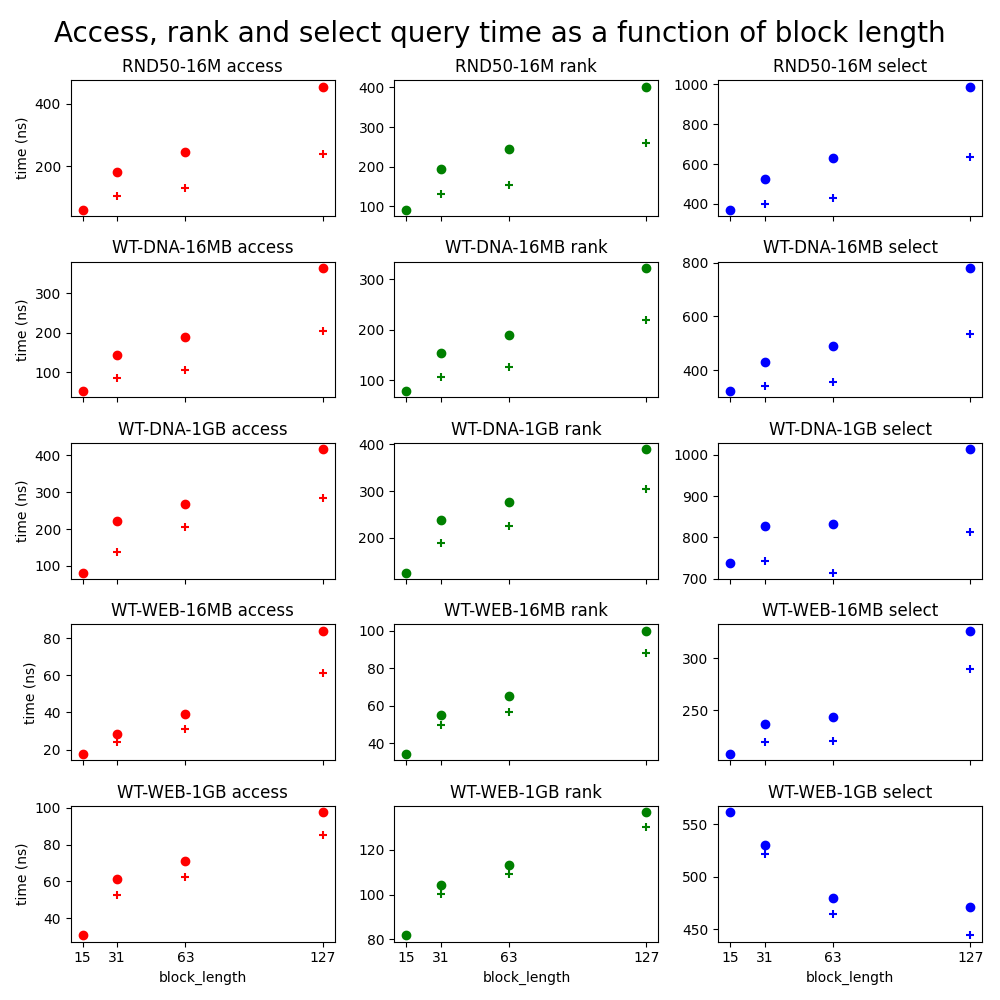
\includegraphics[width=\textwidth, height=0.7\textheight]{images/benchmark_sdsl_new_method}
	}
	\caption[TODO]{\texttt{SDSL} benchmark measuring the query time of $\access$, $\rank$ and $\select$
	and its dependence on the block length across various data types. Our implementations are marked
	by cross.
	}
	\label{obr:benchmark_sdsl_new_method}
\end{figure}

There are several interesting things to observe in these results: Our new implementation
beats older implementation on almost all block lengths and all types of data. Note that the difference is more
visible on random and DNA data. On web data, however, the difference is less noticeable. We attribute
this behaviour to the fact, that was observed by creators of this dataset -- the number of
uniform blocks (full of either zeroes or ones) is much bigger in \texttt{WT-WEB} than in \texttt{WT-DNA}.
For block length 63, they observed that \texttt{WT-WEB-1GB} contains 84\% of uniform blocks compared to 28\% in
\texttt{WT-DNA}. As the uniform blocks are decoded trivially in both implementations, this makes less opportunities
for our implementation to save time.

Another visible pattern is that with increasing block length, the query time generally goes up as decoding takes
more and more time. On the other hand, on $\select$ in \texttt{WT-WEB} data, we can see that at the beginning
the query time decreases with increasing block length. Similar behaviour on this data was observed by
\cite{gog2014optimized} and attributed to the faster binary search in precomputed $\rank$ values offsetting the
growing decoding time.

Overall, we saved almost 50\% of time on $\access$, $\rank$ and $\select$ over randomly generated data,
and close to 50\% of time on \texttt{WT-DNA} data when compared to the baseline implementation. Our results
are positive also on \texttt{WT-WEB}, particularly for block length 127. This block length is particularly
faster in our implementation and we argue this could be also due to the inefficiencies in \texttt{SDSL}s
implementation of 128-bit integer but also due to the fact, that after dividing the problem into subproblems,
we continue to work with 64-bit integers which are much faster on current machines.

\paragraph{Bit vector in FM-index}

Even if the previous benchmark was done on realistic data, we wanted to test our implementation in
a practically useful application. We benchmarked our bit vector as a part of Huffman shaped
wavelet tree used inside of the FM-index. Implementation of FM-index in \texttt{SDSL}, as most
of the other implementations, provides mainly 3 methods:
\begin{itemize}
	\item $\countOp(P)$ -- returns the number of occurrences of $P$ in text $T$,
	\item $\locateOp(P)$ -- returns all positions of pattern $P$ in text $T$,
	\item $\extractOp(i, j)$ -- returns the subsequence of $T$ starting on $i$-th and ending on $j$-th index.
\end{itemize}
The reason that the $\extractOp$ method is useful and non-trivial is that FM-index
does not store the original sequence $T$ -- at least not in an easily readable form.

We again used benchmarks provided by $\texttt{SDSL}$ library and tested how the performance
of methods $\countOp, \locateOp$ and $\extractOp$ changes when our bit vector is used. These
benchmarks are run on the data from the \texttt{Pizza\&Chili} dataset and use mainly methodology
proposed by \cite{ferragina2009compressed}. The data we show here are the English texts from
Gutenberg project, source codes and then DNA and protein sequences. In these benchmarks, we used
as a baseline the FM-index version based on block length 15. To provide more context, we also included
version based on the uncompressed bit vector.

To measure performance of $\countOp$, the index over the text is built. Then, random patterns of
various lengths are extracted from the text and subsequently used for benchmarking. Code
that generates these patterns in \texttt{SDSL} is a slight modification of a version provided
by \texttt{Pizza\&Chili} project. We measure the trade-off between space used for the index and the
speed normalized by the total number of symbols contained in all searched patterns. We present the
results in Fig.~\ref{obr:benchmark_sdsl_count}.

We may observe that the speed gain we have measured in the previous benchmarks also translated
to speedup of FM-index operation $\countOp$. On the English dataset, block lengths 127 and 63 have
been able to obtain the speed of the block lengths 63 and 31 provided by \texttt{SDSL}. The biggest
speed up can be observed for 127-bit block -- on English data the time saved is close to 20\%, on
DNA it is roughly 30\% speedup.

On graphs where we can observe the tradeoff between space and time it is important not only to
focus on fastest and most succinct implementations but also on those that are \textit{Pareto optimal}.
This means that certain implementation may not be the fastest or space optimal but to obtain faster
implementation leads to increase in space usage and vice versa.

\begin{figure}
	\centerline{
		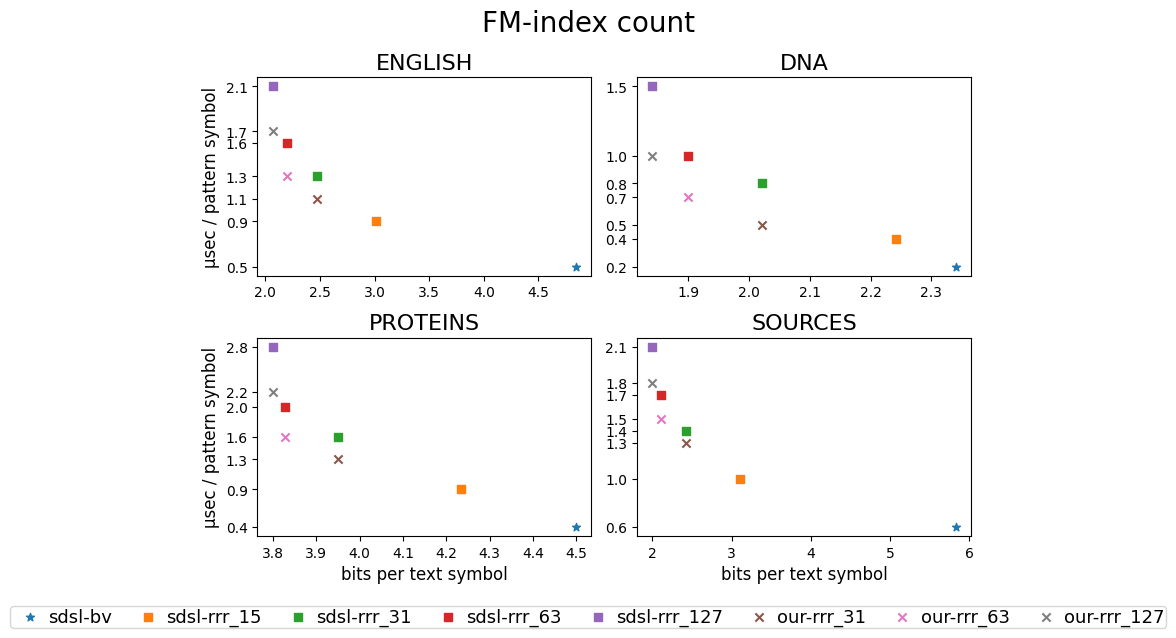
\includegraphics[width=\textwidth, height=0.4\textheight]{images/vysledky_sdsl_count}
	}
	\caption[TODO]{Counting occurrences of patterns in various different texts. Displaying
	the query time per pattern symbol on $y$-axis and the size of the index over the
	text on $x$-axis. Uncompressed bit vector (sdsl-bv) is included for reference. 
	}
	\label{obr:benchmark_sdsl_count}
\end{figure}

For benchmarking of $\extractOp$, \texttt{SDSL} uses a methodology proposed by
\cite{ferragina2009compressed} in Section~5.4. The queries used for benchmarking consist of
numerous substrings of length 512 starting at random positions in text. The additional dimension
of FM-index that is tested in this benchmark is sampling rate of suffix array and inverse suffix
array. This is a parameter that can be used to trade-off between the speed of FM-index and
its memory usage. Options for this sampling ratio are by default the powers of 2 from 4 up to
256. We only show the results for a sampling rate 16 in Fig.~\ref{obr:benchmark_sdsl_extract},
however, note that the trends that can be observed in these results are also visible for every
sampling rate.

We may observe similar speedup as for $\countOp$ method. The visible difference is slightly
bigger speedup on Sources for block length 31. On the DNA data, the speedup is hitting again 30\%.

\begin{figure}
	\centerline{
		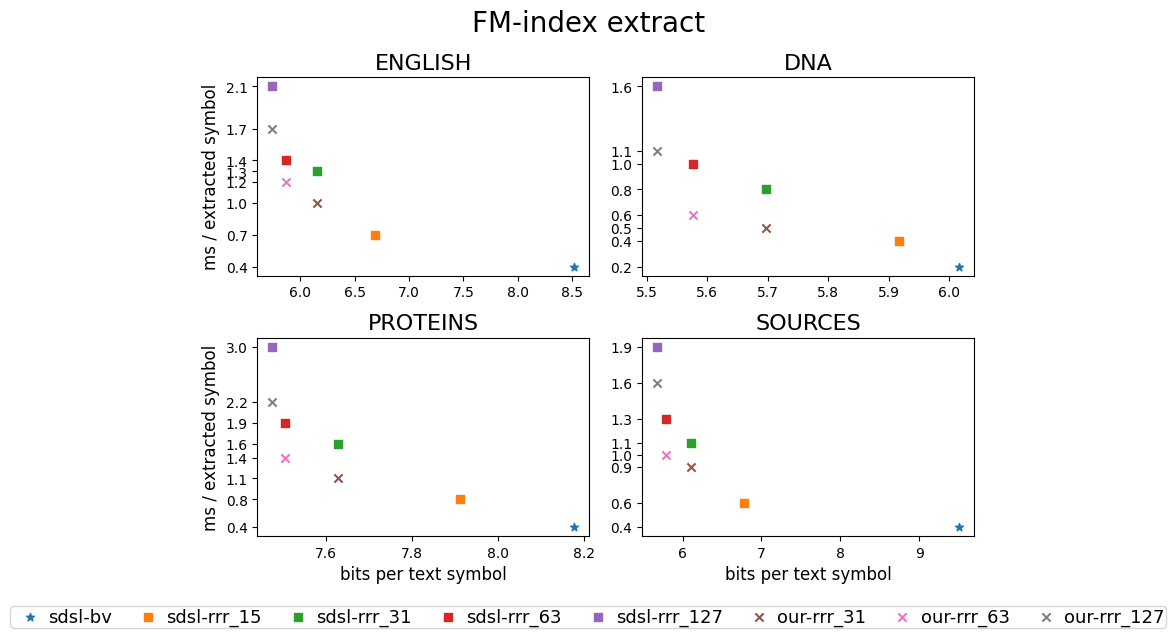
\includegraphics[width=\textwidth, height=0.4\textheight]{images/vysledky_sdsl_extract}
	}
	\caption[TODO]{Extracting parts of the represented text. Displaying
	the query time per extracted symbol on $y$-axis and the size of index over the text on $x$-axis.
	Uncompressed bit vector (sdsl-bv) is included for reference. 
	}
	\label{obr:benchmark_sdsl_extract}
\end{figure}

Benchmarking of operation $\locateOp$ again uses a methodology proposed by \cite{ferragina2009compressed} 
in Section~5.3. This consists of locating random patterns of length 5 in the text such
that in total 2--3 millions of occurrences are found in the text. We present the results
obtained in Fig.~\ref{obr:benchmark_sdsl_locate}.

The results are very strong for DNA, Protein and Sources datasets but even on English, where
our method performed the worst we can observe 10--20\% speed up on every block length.

\begin{figure}
	\centerline{
		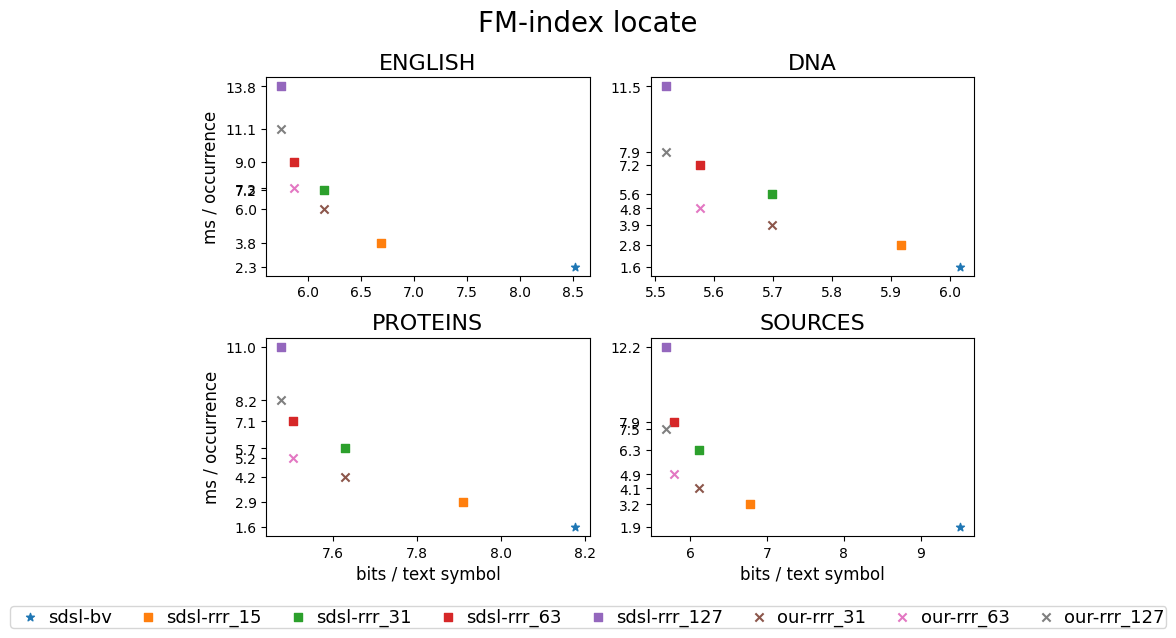
\includegraphics[width=\textwidth, height=0.4\textheight]{images/vysledky_sdsl_locate}
	}
	\caption[TODO]{Locating occurrences of patterns in the represented text. Displaying
	the query time per occurrence for various block sizes and the size of index over the
	text.
	}
	\label{obr:benchmark_sdsl_locate}
\end{figure}

\paragraph{Correctness}

On top of making sure that our solution is as fast as possible we also wanted to make sure it is
correct. Mainly, we used two types of tests for this purpose. The first are the tests of $\access$,
$\rank$ and $\select$ functionality in \texttt{SDSL} that run more on smaller bit sequences
but cover special cases such as bit vector full of zeroes/ones and certain special patterns
that are not encountered often in practice. The second type of tests used was the benchmark
running on wavelet tree built over the \texttt{WT-DNA} and \texttt{WT-WEB} data. Alongside
the individual timings, this benchmark produces, as a checksum, sum of all the results of the
$\access$, $\rank$ and $\select$ queries. These checksums can be compared between our and original
implementation to make sure that our implementation is giving the correct results.

\section{Hybrid encoding}

Let us now present our implementation of the hybrid encoding. In the previous chapter, we
proposed two variants of hybrid encoding -- one-sided and two-sided version. Both of these
were based on the idea not to encode blocks that are rare. This in turn reduced the number
of classes and we  have been able to save space on bits used for blocks classes. On the other
hand, these two versions differed in decision, which blocks are not encoded but just saved in
ther original representation. The first solution treated differently just blocks with higher
number of ones. The second, was focused on balanced sequences and treated differently blocks
that have roughly the same number of zeroes and ones.

\subsection{Implementation}

Implementation of the hybrid encoding required changes to more than only encoding and decoding
routines. The first necessary change is addition of hybrid cutoff parameter $c_k$
to the \verb'rrr_vector' class. The second is reimplementation of function
\texttt{space\_for\_bt(c)} that is used in \texttt{SDSL} to get the number of bits that are
needed to store offset of block with class $c$. The third change, most impactful on a runtime
of \verb'rrr_vector', relates to the way how we work with superblocks.

When computing $\rank$ of a bit in particular block, we can still binary search for
the superblock where the $i$-th one is located. Then, to linearly search for a result
inside of the superblock, we previously needed only information from the array of classes $C$.
This is because $C$ stores the number of ones in the blocks and we can linearly
search for the answer using its successive entries. We skip over the blocks inside of the
superblock until we find the block where the result is located. This block needs to be decoded
and only then we find answer to $\rank$ inside of a single block. To locate the beginning of this
smaller block, we take the memory offset of the superblock in $O$ and add the memory offset of this
block from the beginning of superblock. This can be counted along with the linear search for $\rank$
result. The simplified implementation of the $\rank$ in \texttt{SDSL} is in Listing~\ref{code:rank_before}.

With hybrid implementation, however, we are not able to linearly scan through the superblock only
using information contained in $C$. This is because now, for some classes, $C$ does not
store the number of ones in the block. Thus when we are linearly searching for the result
of $\rank$ query along the superblock, we need to also from time to time access $O$ to count
number of ones for some block. This creates additional memory accesses that may slow down the
hybrid implementation. The new version of implementation, adapted to the hybrid encoding is in
Listing~\ref{code:rank_after}.

In both versions of hybrid implementation, we introduced cutoff parameter $c_k$ to the
class \verb'rrr_vector'. Its meaning is that exactly $c_k$ classes are represented
as before and the rest of them is represented using a single value. In the first version,
these are classes bigger or equal than $c_k$. In the second version, these are classes
from range \texttt{cut\_from} up to and including \texttt{cut\_to}. For certain $c_k$,
we need then $\lg (c_k+1)$ bits of space to represent a single class.

\lstset{language=C++,caption={Rank query, SDSL implementation},label=code:rank_before}
\begin{lstlisting}
int rank(int i) {
	int block_idx = i/BLOCK_SIZE;
	int superblock_index = block_idx/BLOCKS_PER_SUPERBLOCK;
	int offset = P[superblock_idx]; // precomputed offset into O
	int rank  = R[superblock_idx]; // precomputed rank for superblock
	for (int j = superblock_idx*BLOCKS_PER_SUPERBLOCK; j < block_idx; ++j) {
		uint16_t c = C[j];
		rank  += c;
		offset += rrr_helper::space_for_class(c);
	}
	uint16_t off = i % BLOCK_SIZE;
	if (!off) {
		return rank;
	}
	uint16_t c = C[block_idx];

	uint16_t block_length = rrr_helper::space_for_class(c);
	uint32_t o = rrr_helper::get_blocks_offset(O, offset, block_length);
	uint16_t popcnt  = __popcount(rrr_helper::nr_to_bin(c, o) << (32-off));
	return rank + popcnt;
}
\end{lstlisting}

\lstset{language=C++,caption={Rank query, hybrid implementation (one-sided)},label=code:rank_after}
\begin{lstlisting}
int rank(int i) {
	int block_idx = i/BLOCK_SIZE;
	int superblock_index = block_idx/BLOCKS_PER_SUPERBLOCK;
	int offset = P[superblock_idx];
	int rank  = R[superblock_idx]; // precomputed rank for superblock
	for (int j = superblock_idx*BLOCKS_PER_SUPERBLOCK; j < block_idx; ++j) {
		uint16_t c = C[j];
		if (c >= c_k) {
			uint32_t o = rrr_helper::get_blocks_offset(O, offset, BLOCK_SIZE);
			rank += __popcount(btnr);
		}
		else {
			rank  += c;
		}
		offset += rrr_helper::space_for_class(r);
	}
	uint16_t off = i % BLOCK_SIZE;
	if (!off) {
		return rank;
	}
	uint16_t c = C[block_idx];

	uint16_t block_length = rrr_helper::space_for_class(c);
	uint32_t o = rrr_helper::get_blocks_offset(O, offset, block_length);
	uint16_t popcnt  = __popcount(rrr_helper::nr_to_bin(c, o) << (32-off));
	return rank + popcnt;
}
\end{lstlisting}

\paragraph{Two sided version}

The biggest notable difference from the previous version of hybrid encoding are the two
helper functions that are used for mapping or as we call it compressing and decompressing
the blocks class before any of its use. We present these methods in listing \ref{code:hybrid_valley_compress},
and \ref{code:hybrid_valley_decompress}. To choose for particular $c_k$, which $c_k$ classes we are
going to represent in a standard way, we set
$$\text{cut\_from} = \floor{(c_k+1)/2}\qquad \text{cut\_to} = b-\text{cut\_from}+1.$$

\lstset{language=C++,caption={Compressing blocks class},label=code:hybrid_valley_compress}
\begin{lstlisting}
int compress_class(int k) {
	if (!is_hybrid_impl) return k;
	if (k < cut_from) {
		return k;
	}
	else if (k <= cut_to) {
		return cutoff;
	}
	else {
		return k-(cut_to-cut_from+1);
	}
}
\end{lstlisting}

\lstset{language=C++,caption={Decompressing blocks class},label=code:hybrid_valley_decompress}
\begin{lstlisting}
int decompress_class(int k) {
	if (!is_hybrid_impl) return k;
	if (k < cut_from) {
		return k;
	}
	else if (k == cutoff) {
		return cut_to;
	}
	else {
		return k+(cut_to-cut_from+1);
	}
}
\end{lstlisting}

\subsection{Experimental results}

The goal of the first benchmark was to observe, how the one-sided version of hybrid encoding
behaves on randomly generated sequences with fixed percentage of ones. The reason behind this
test is that bit vector implementations based on RRR do not perform very well on this type of
sequences and are often dominated by sparse bit vector implementations.

We generated a random sequence of bits containing 5\% of ones and compared hybrid implementation
with our original RRR implementation and also sparse bit vector provided by \texttt{SDSL}. We
present the results in Fig.~\ref{obr:vysledky_hybrid_artif}. We may observe that our implementation
was already competitive with sparse array for $\access$ and $\rank$. Hybrid encoding only amplified
these differences. However, on $\select$ where our implementation was dominated by sparse array,
these differences were not completely overcome by hybrid implementation. We can, however, conclude
that hybrid version of 63 and 127-bit block created new viable alternatives, most importantly for
$\select$ method and 127-bit block where it move the representation very close to optimal 0.29
bits per one bit in original sequence.

We tested our second version of hybrid encoding on the previously used datasets \texttt{WT-DNA}
and \texttt{WT-WEB}. The graph comparing results for classic bit vectors and hybrid bit vectors
can be observed in Fig.~\ref{obr:vysledky_sdsl_hybrid}. The results of our hybrid implementation
are not very promising on these data, except for the $\access$. The reason why the results are
better for $\access$ is that hybrid implementation creates additional memory accesses when answering
$\rank$ and $\select$ as we described in the previous subsection. 

To test if our hybrid implementation could be used in the practice, we benchmarked FM-index
implementation of method $\countOp$, with hybrid bit vector used inside of the Huffman shaped
wavelet tree. The results are shown in Fig~\ref{obr:benchmark_sdsl_hybrid_count}.

\begin{figure}
	\centerline{
		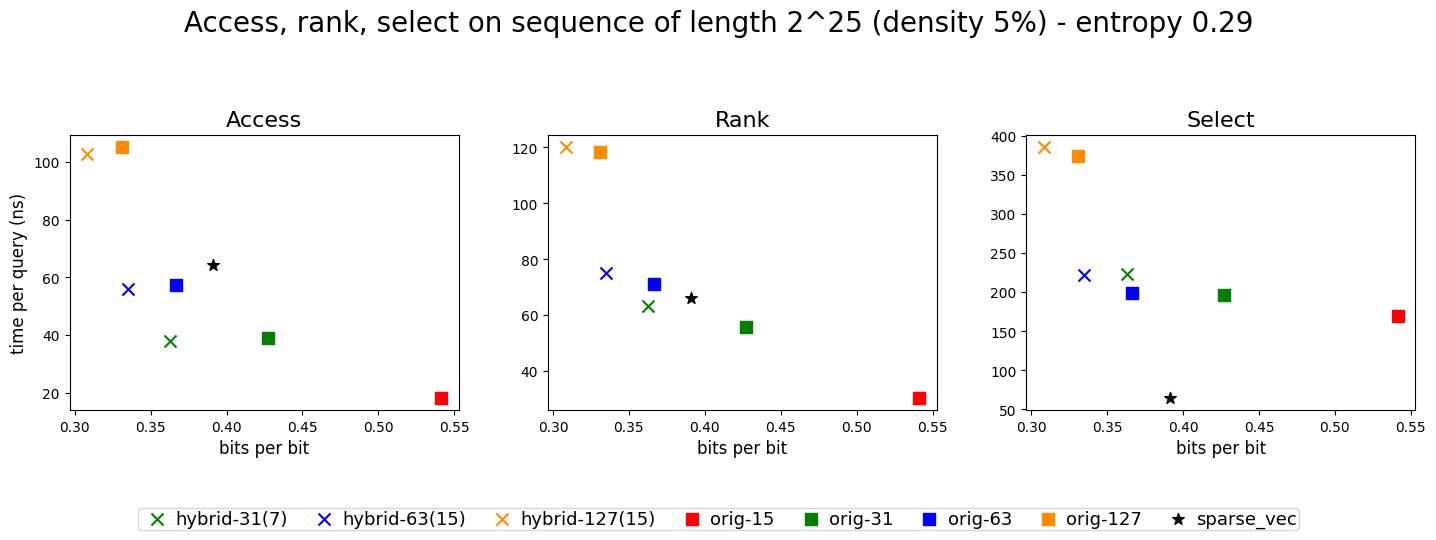
\includegraphics[width=\textwidth, height=0.27\textheight]{images/vysledky_hybrid_artif}
	}
	\caption[TODO]{Timing of $\access$, $\rank$ and $\select$ methods over the randomly generated
	sequence with 5\% of ones in it. Comparison of standard implementation and our hybrid encoding
	marked with cross. For reference, we included sparse vector implementation. We may observe how
	implementations get closer to the entropy lower bound (0.29) with increasing block size. Name
	$\texttt{hybrid-}x\texttt{(}y\texttt{)}$ denotes implementation of block size $x$ with cutoff $y$.
	}
	\label{obr:vysledky_hybrid_artif}
\end{figure}

\begin{figure}
	\centerline{
		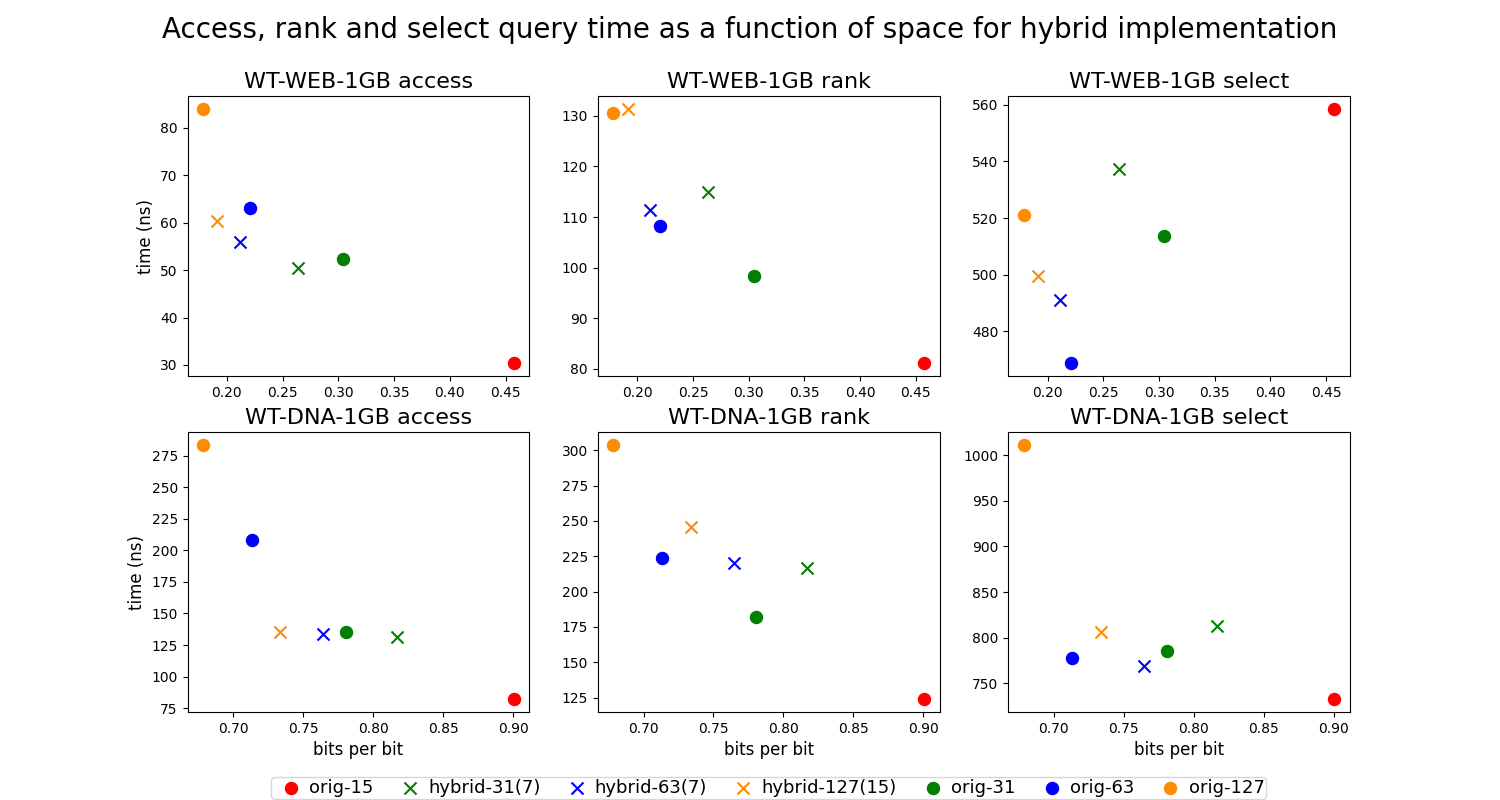
\includegraphics[width=\textwidth, height=0.35\textheight]{images/vysledky_sdsl_hybrid}
	}
	\caption[TODO]{This graph is showing the results of benchmark of $\access$, $\rank$ and $\select$
	queries over bit vectors from wavelet tree over DNA sequence data \texttt{WT-DNA} and XML bibliographic
	data \texttt{WT-WEB}. On $x$-axis is the space usage of the particular representation and on $y$-axis
	the average query time for the respective operation. Original implementation is denoted by dots. These
	are our implementations except for the 15-bit version based on the table lookup provided by \texttt{SDSL}.
	Every cross symbols hybrid implementation with particular cutoff. The same block size is denoted by a
	single color. Name $\texttt{hybrid-}x\texttt{(}y\texttt{)}$ denotes implementation of block size $x$ with
	cutoff $y$.
	}
	\label{obr:vysledky_sdsl_hybrid}
\end{figure}

\begin{figure}
	\centerline{
		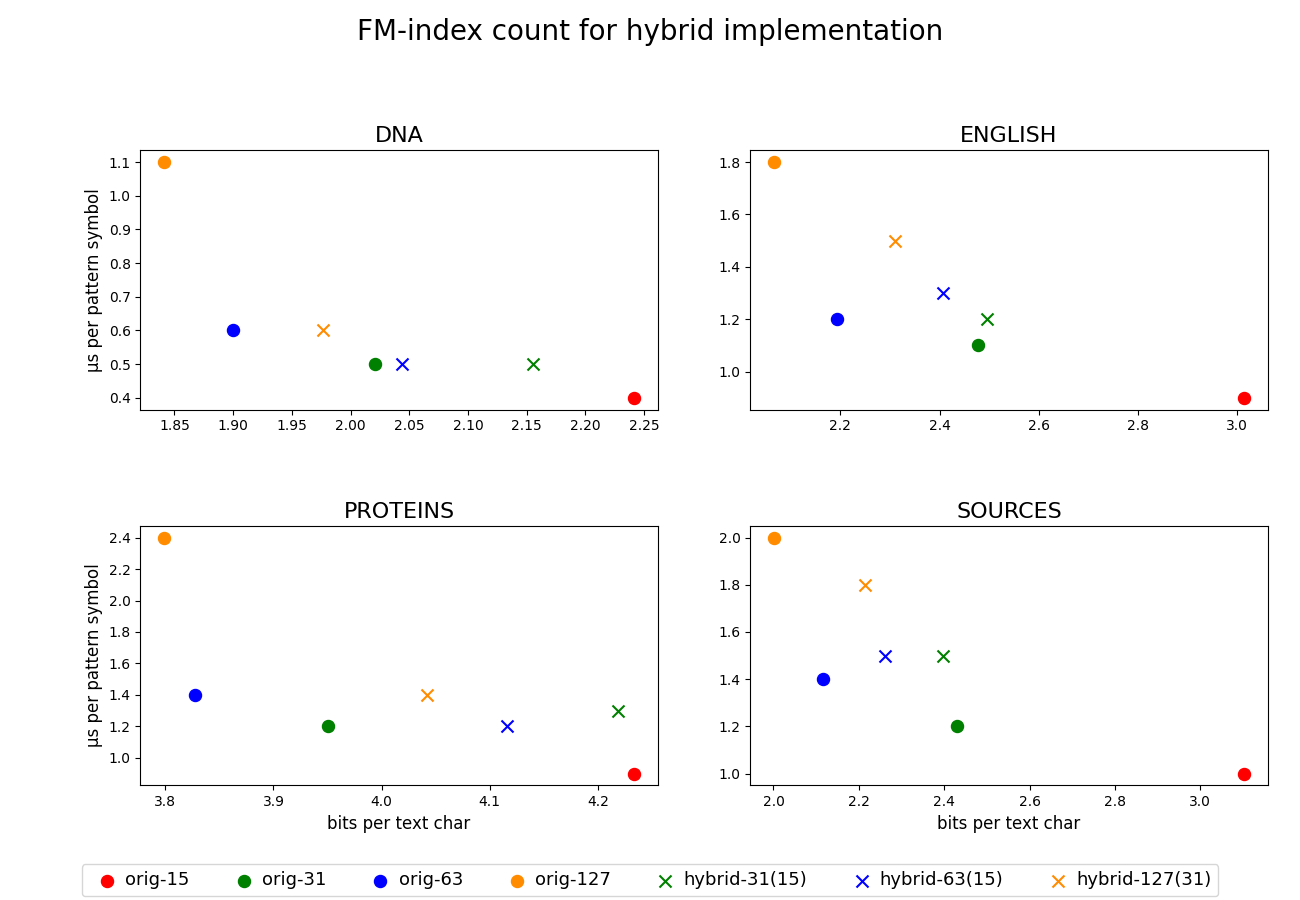
\includegraphics[width=\textwidth, height=0.5\textheight]{images/vysledky_sdsl_hybrid_count}
	}
	\caption[TODO]{Results of benchmark of $\countOp$ operation on FM-index.
	}
	\label{obr:benchmark_sdsl_hybrid_count}
\end{figure}

%\begin{figure}
%	\centerline{
%		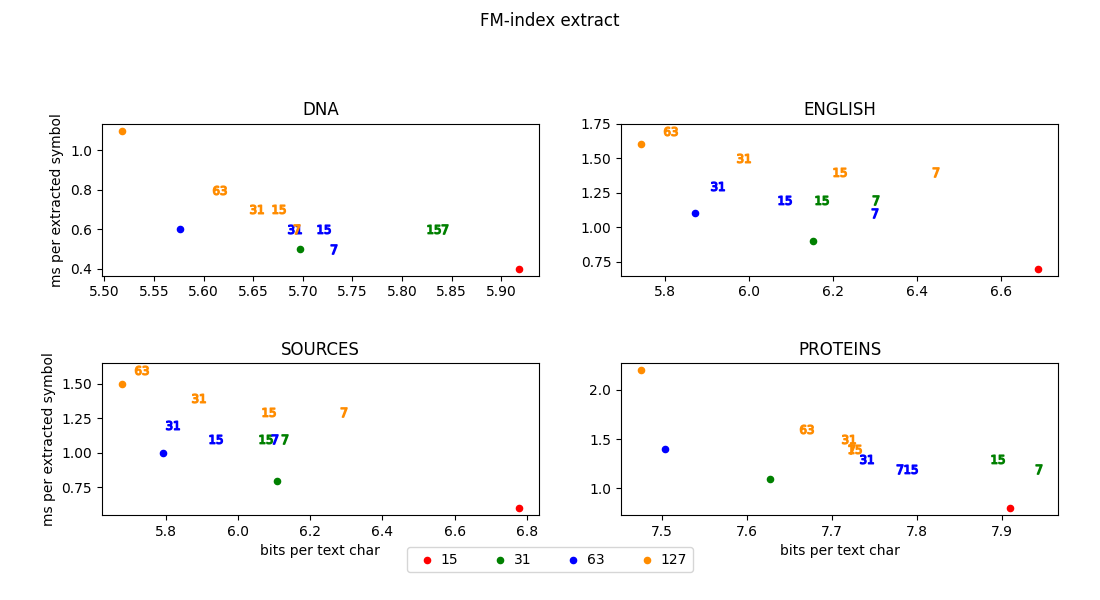
\includegraphics[width=\textwidth, height=0.4\textheight]{images/vysledky_sdsl_hybrid_extract}
%	}
%	\caption[TODO]{TODO
%	}
%	\label{obr:benchmark_sdsl_hybrid_extract}
%\end{figure}

%Before implementing our second version of hybrid encoding, we have been interested in a potential
%space saving on some real-life data so we analyzed what is the space saved when using hybrid encoding
%on a data \texttt{WT-WEB-1GB} and \texttt{WT-DNA-1GB}. The results in Fig.~\ref{obr:hybrid_space_saved}
%show, that there is a potential to save some space for certain cutoff values.

%\begin{figure}
%	\centerline{
%	\begin{tabular}{|l|l|r|}
%		\multicolumn{3}{c}{WT-DNA-1GB} \\
%		\hline
%		Block size 			& $c_k$					&  space used by hybrid \\
%		\hline
%		\multirow{2}{*}{31} & 7                  	&  90\%  \\
%							& 15  					&  97\%  \\
%		\hline
%		\multirow{3}{*}{63} & 7                 	&  93\%  \\
%							& 15                 	&  97\%  \\
%							& 31  					&  100\%  \\
%		\hline
%		\multirow{4}{*}{127}& 7                 	&  99\%  \\
%							& 15                 	&  99\%  \\
%							& 31  					&  101\%  \\
%							& 63  					&  102\%  \\
%		\hline
%	\end{tabular}
%	\hspace{3em}
%	\begin{tabular}{|l|l|r|}
%		\multicolumn{3}{c}{WT-WEB-1GB} \\
%		\hline
%		Block size 			& $c_k$					&  space used by hybrid \\
%		\hline
%		\multirow{2}{*}{31} & 7                  	&  73\%  \\
%							& 15  					&  85\%  \\
%		\hline
%		\multirow{3}{*}{63} & 7                 	&  78\%  \\
%							& 15                 	&  84\%  \\
%							& 31  					&  91\%  \\
%		\hline
%		\multirow{4}{*}{127}& 7                 	&  94\%  \\
%							& 15                 	&  94\%  \\
%							& 31  					&  94\%  \\
%							& 63  					&  95\%  \\
%		\hline
%	\end{tabular}
%	}
%	\caption[TODO]{TODO.
%	}
%	\label{obr:hybrid_space_saved}
%\end{figure}
